\documentclass{article}

\usepackage{fontspec}                % font for emoji
\newfontfamily\DejaSans{DejaVu Sans}

\usepackage{arxiv}

\usepackage[utf8]{inputenc} % allow utf-8 input
\usepackage[T1]{fontenc}    % use 8-bit T1 fonts
\usepackage{hyperref}       % hyperlinks
\usepackage{url}            % simple URL typesetting
\usepackage{booktabs}       % professional-quality tables
\usepackage{amsfonts}       % blackboard math symbols
\usepackage{nicefrac}       % compact symbols for 1/2, etc.
\usepackage{microtype}      % microtypography
\usepackage{lipsum}		    % Can be removed after putting your text content
\usepackage{graphicx}
\usepackage{natbib}
\usepackage{doi}            % hyperlink to doi.org
\usepackage{enumitem}       % itemize settings
\usepackage{cleveref}       % reference section with capital letter
\usepackage{xcolor}         % additional colors for hypersetup
\usepackage{booktabs}       % beauful tables
\usepackage{caption}        % table caption margin
\usepackage{subcaption}     % images next to each other
\usepackage{placeins}       % floatbarrier
\usepackage[outputdir=build]{minted} % code insertion

\captionsetup[table]{skip=10pt}          % table caption margin
\setlist[itemize]{noitemsep, topsep=0pt} % no space between itemize
\hypersetup{
    colorlinks=true,
    citecolor=violet,
    linkcolor=violet,
    filecolor=violet,      
    urlcolor=black,
}

\title{A Hybrid Approach for News Recommender System using Optimization Methods}

%\date{September 9, 1985}	% Here you can change the date presented in the paper title
%\date{} 					% Or removing it

\author{
    {
\includegraphics[scale=0.07]{./images/spbu.png}\hspace{1mm}Alexander Smirnov}\\
	Department of Information and Analytical Systems\\
	Saint Petersburg State University\\
	Russia, Saint Petersburg\\
	\texttt{ru.alexander.smirnov@gmail.com} \\
	\And
	{
\includegraphics[scale=0.07]{images/spbu.png}\hspace{1mm}Elena Mikhailova} \\
	Department of Information and Analytical Systems\\
	Saint Petersburg State University\\
	Russia, Saint Petersburg\\
	\texttt{e.mikhaylova@spbu.ru} \\
	%% \AND
	%% Coauthor \\
	%% Affiliation \\
	%% Address \\
	%% \texttt{email} \\
	%% \And
	%% Coauthor \\
	%% Affiliation \\
	%% Address \\
	%% \texttt{email} \\
	%% \And
	%% Coauthor \\
	%% Affiliation \\
	%% Address \\
	%% \texttt{email} \\
}

% Uncomment to remove the date
%\date{}

% Uncomment to override  the `A preprint' in the header
%\renewcommand{\headeright}{Technical Report}
%\renewcommand{\undertitle}{Technical Report}
\renewcommand{\shorttitle}{Recommender System}

\hypersetup{
    pdftitle={A hybrid approach for news recommender system using optimization methods},
    pdfsubject={recommender systems},
    pdfauthor={Alexander Smirnov, Elena Mikhailova},
    pdfkeywords={Recommender Systems, Optimizations},
}

\begin{document}

\maketitle

\begin{abstract}


    Recommender system is an essential part of any social media application. Most recommender systems now use a hybrid approach, combining collaborative filtering, content-based filtering, and other approaches. Most common problems in the field of hybrid recommenders are cold start and data sparsity \citep{overview}. In this paper we address the abovementioned problems by proposing a hybrid weighted news recommender system which combines different approaches.

\end{abstract}


\keywords{hybrid recommender systems \and content-based recommender \and collaborative recommender \and optimizations}



\section{Introduction}




    Recommender system is a crucial part of every application that operates with content and user activity. Enormous amount of information leads to the problem that user is not able to find relevant content.

    Recommender systems have been studied to present items, such as movies, music, and books \citep{movies} \citep{films} \citep{books}. The term now has a broader connotation, describing any system that produces individualized recommendations as output or has the effect of guiding the user in a personalized way to interesting or useful objects in a large space of possible options. Such systems have an obvious appeal in an environment where the amount of on-line information vastly outstrips any individual’s capability to survey it.

    Recommender systems are now an integral part of some e-commerce sites such as Amazon.com and CDNow \citep{commerce}. It is the criteria of ’individualized’ and ’interesting and useful’ that separate the recommender system from information retrieval systems or search engines \citep{coin}. The semantics of a search engine are ’matching’: the system is supposed to return all those items that match the query ranked by degree of match.  Techniques such as relevance feedback enable a search engine to refine its representation of the user’s query, and represent a Simple form of recommendation.

    Field of news recommendation has its own specific: news are getting old really fast and they don't need to be recommended.

     There are three main types of recommendation methods: memorybased, model-based, and hybrid \citep{survey}. Memory-based methods \citep{memory} usually use similarity metrics to obtain the distance between two users or two items. Model-based methods use demographic, content, or aggregated information to create a model that generates recommendations. Hybrid \citep{combining} methods combine different types of recommenders to gain better performance.

    Common approaches, such as collaborative filtering, have their own problems: cold start, scalability and data sparsity. Content-based approaches suffer from the fact that we have to somehow represent recommended item in feature space.

    So we are going to present a hybrid recommender system.
    
    To be consistent during the paper we list some domain specific vocabulary with their meanings:

        \begin{itemize}
            \item Rating: expression or preference

                \begin{itemize}
                    \item explicit (direct from user, e.g. user rated film)
                    \item implicit (inferred from user activity, e.g. user stopped watching movie after 5 minutes)
                \end{itemize}
            \item Prediction: estimate of preference
            \item Recommendation: selected items for user
            \item Content: attributes, text, etc; everything about item
        \end{itemize}


    The remainder of this paper is organized as follows:
    
        \begin{itemize}
            \item \Cref{sec:related} describes the relevant related work
            \item \Cref{sec:input} describes input data
            \item \Cref{sec:overview} explains our modular design and architecture
            % \item \Cref{sec:implementation} describes the implementation of the algorithms in a real system
            \item \Cref{sec:evaluation} provides tests and experiments validating
our system’s results
            \item \Cref{sec:further} explains future work
            \item \Cref{sec:summary} presents conclusions
        \end{itemize}



\section{Related work}
\label{sec:related}

According to the study \citep{progress}, deep learning techniques are not supposed to beat conceptually and computationally simpler algorithms, so we won't touch them.

Our goal is to choose optimal algorithm for each of the following tasks:

\begin{itemize}
    \item \textbf{Collaborative filtering}: generating predictions about the interests of a user by collecting preferences or taste information from other users. It is based on the assumption that if a person A has the same opinion as a person B on an issue, A is more likely to have B's opinion on a different issue than that of a randomly chosen person; there were many studies on this topic, but paper \citep{evaluation} proves that well-tuned basic SVD++ approach beats newely presented algorithms
    \item \textbf{Content-based filtering}: is based on the assumption that people who liked items with certain attributes in the past, will like the same kind of items in the future as well. It makes use of item features to compare the item with user profiles and provide recommendations
    \item \textbf{Session filtering}: is selecting cadidates based on user's activity on current session
    \item \textbf{Popularity filtering}: uses information such as number of views, shows, comments, etc.
    \item \textbf{Demographic filtering}: uses demographic data such as age, gender, education, etc. for identifying categories of users
    \item \textbf{Time-based filtering}: ranking news is a way that more recent items have higher scores
\end{itemize}

Also there is several ways \citep{survey1} to combine recommenders between each other:

\begin{itemize}
    \item \textbf{Weighted}: The scores (or votes) of several recommendation techniques are.combined together to produce a single recommendation
    \item \textbf{Switching}: The system switches between recommendation techniques depending on the current situation
    \item \textbf{Mixed}: Recommendations from several different recommenders are presented at the same time
    \item \textbf{Feature combination}: Features from different recommendation data sources are thrown together into a single recommendation algorithm
    \item \textbf{Cascade}: Features from different recommendation data sources are thrown together into a single recommendation algorithm 
    \item \textbf{Feature augmentation}: Output from one technique is used as an input feature to another
    \item \textbf{Meta-level}: The model learned by one recommender is used as input to another
\end{itemize}


We face the problem that millions of news are theoretically suitable for being recommended, so it is not correct to use abovementioned methods on such large corpus of data. Instead, as stated in \citep{youtube} paper, we want to implement \texttt{candidate generation} $\to$ \texttt{ranking} pipeline to reduce number of candidates.


\section{Input data}
\label{sec:input}

As we solving domain specific task, we have domain specific data.
Out data consist of information about news, so it includes following tables:

\subsection*{metadata}

The metadata about news. Here we have an \textit{item\_id} column, which stands for unique item indentifier, afterwards \textit{date}, that shows when this item was released. The \textit{source\_id} column stands for id of a publisher of this news item. \textit{category} column means category of current news item. This category is taken from news text by keywords.

\begin{table}[h]
    \centering
    % \resizebox{\textwidth}{!}{
    \begin{tabular}{ccccc}
        \toprule

        \emph{item\_id} & \emph{date} & \emph{source\_id} & \emph{category}\\\midrule

        1 & 2021-01-08 22:08:39 & 9  & politics, conflicts\\
        2 & 2021-01-09 10:28:58 & 5  & IT, social media\\
        3 & 2021-01-09 14:20:34 & 12 & accident\\
        \vdots & \vdots & \vdots & \vdots \\\bottomrule
    \end{tabular}
    % }

    \caption{news metadata}
    \label{tab:meta}
\end{table}


% \begin{itemize}
%     \item \emph{source\_id}: source of news item
% \end{itemize}


\subsection*{content}

Content table hold news texts in a \textit{news\_content} column. This is the primary information that is being used by our recommender system, because we are able to extract a lot of valuable data from text, such as topics.

\begin{table}[h]
    \centering
    \resizebox{\textwidth}{!}{
    \begin{tabular}{cll}    \toprule

        \emph{item\_id} &  \emph{news title} & \emph{news content} \\\midrule

    1  &  Azerbaijan denies reports on construction of Turkish air bases in the country & Information that Turkey will create air bases ...        \\
    2  &  Durov announced the massive transition of WhatsApp users to Telegram          & Telegram developer Pavel Durov said in his channel ...   \\
    3  &  Passenger plane that disappeared from radar crashed                           & Passenger plane taking off from Jakarta, disappeared ... \\
    \vdots & \vdots & \vdots \\\bottomrule
    \end{tabular}
    }
    \caption{news item}
    \label{tab:item}
\end{table}

\subsection*{shows \& views}

As we operate with user activity we should have user logs, such as what items were clilcked at what time, so we have separate table that contains this information.    \emph{shows} stands for \emph{item\_id} was shown to the \emph{user\_id}, \emph{views} is if \emph{item\_id} was clicked by the \emph{user\_id}.

\begin{table}[h]
    \parbox{.45\textwidth}{
        \centering
        \begin{tabular}{ccc}
            \toprule

            \emph{user\_id} & \emph{item\_id} \\\midrule
            10 & 1  \\
            10 & 2  \\
            23 & 1  \\
            23 & 3  \\
            23 & 2  \\
            38 & 3  \\
            38 & 1  \\
            \vdots & \vdots  \\\bottomrule
        \end{tabular}
        \caption{news shows}
        \label{tab:show}
    }
    \hfill
    \parbox{.45\textwidth}{
        \centering
        \begin{tabular}{ccc}
            \toprule

            \emph{user\_id} & \emph{item\_id} \\\midrule
            10 & 1  \\
            10 & 2  \\
            23 & 1  \\
            38 & 3  \\
            \vdots & \vdots  \\\bottomrule
        \end{tabular}
        \caption{news views}
        \label{tab:view}
        }
\end{table}   


% \begin{itemize}
%     \item \emph{shows}: if \emph{item\_id} was shown to the \emph{user\_id}
%     \item \emph{views}: if \emph{item\_id} was clicked by the \emph{user\_id}
% \end{itemize}



\subsection*{emotions \& comments}

We have an explicit feedback that user may leave on a news if he wants to. These options includes leaving emoji, which is one of \{{\DejaSans 😄, 😲, 😞, 😡, ♥ }\} or comment, which we can analyze afterwards.

\begin{table}[h]
    \parbox{.45\textwidth}{
        \centering
        \begin{tabular}{ccc}
            \toprule

            \emph{user\_id} & \emph{item\_id} & \emph{emotion\_id} \\\midrule
            10 & 1 & 1  \\
            10 & 2 & 3        \\
            23 & 1 & 3        \\
            38 & 3 & 2        \\
            \vdots & \vdots & \vdots  \\\bottomrule

        \end{tabular}
        \caption{users' emotions}
        \label{tab:emotion}
    }
    \hfill
    \parbox{.45\textwidth}{
        \centering
        \resizebox{0.45\textwidth}{!}{
        \begin{tabular}{ccc}
            \toprule

            \emph{user\_id} & \emph{item\_id} & \emph{comment} \\\midrule
            10 & 1 & that's great  \\
            10 & 1 & wish it will continue        \\
            23 & 2 & whatsapp is not competetive anymore        \\
            \vdots & \vdots & \vdots  \\\bottomrule

        \end{tabular}
    }
        \caption{users' comments}
        \label{tab:comment}
        }
\end{table}   

% \begin{itemize}
%     \item \emph{emotion\_id}: one of \{{\DejaSans 😄, 😲, 😞, 😡, ♥ }\}
% \end{itemize}


% \FloatBarrier


\subsection*{users' subscriptions}

Each piece of news is being posted by some feed and user have an ability to subscribe to the feed. So it may give us useful information if user prefers content from one feed to content to another feed. So following table illustrates if \emph{user\_id} subscribed to the \emph{source\_id}.

\begin{table}[h]
    \centering
    \begin{tabular}{cc}
        \toprule

        \emph{user\_id} & \emph{source\_id} \\\midrule

        10 & 9  \\
        23 & 5  \\
        \vdots & \vdots  \\\bottomrule

    \end{tabular}

    \caption{users' subscriptions}
    \label{tab:subscriptions}
\end{table}


\newpage
\section{Overview of our approach}
\label{sec:overview}

Out goal is to combine state-of-the-art approaches in recommender systems.

Solution consists of 2 parts:

\begin{itemize}
    \item \textbf{Candidate generation}: lowering number of items to recommend. These candidates are intended to be generally relevant to the user with high precision. The candidate generation part only provides broad personalization
    \item \textbf{Ranking}: applying state-of-the-art algorithms to rank candidates generated on previous step
\end{itemize}

Architecture provided below on \cref{fig:architecture}:

\begin{figure}[h]
    \centering
    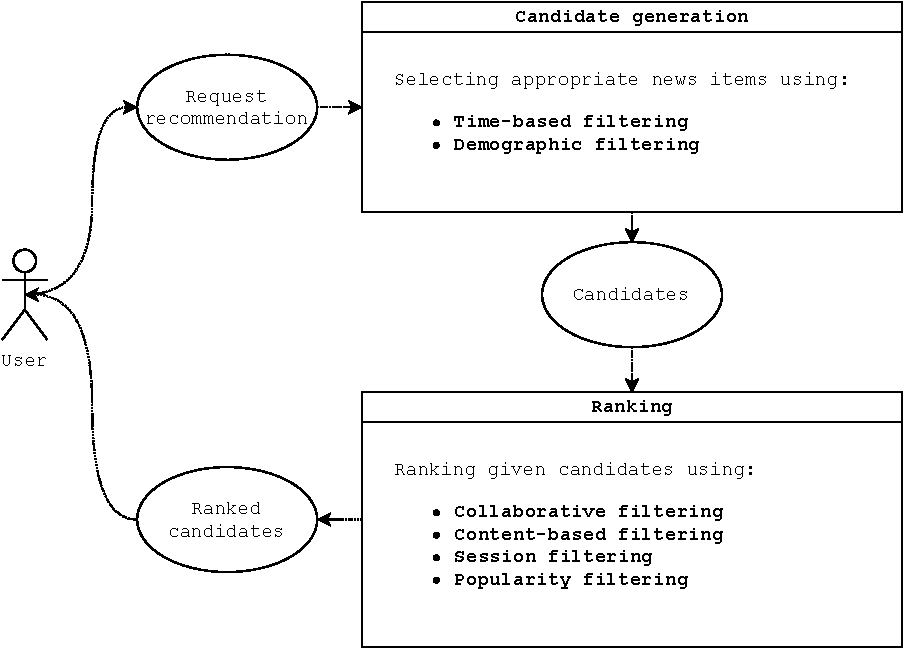
\includegraphics[width=0.8\textwidth]{./images/architechture.pdf}
    \caption{architecture}
    \label{fig:architecture}
\end{figure}

Candidate generation stage not only filters items, but also attaches weights to them.

\subsection{Candidate generation components overview}

Goal of candidate generation step is to remove generally irrelevant items so furher algorithms won't suffer from the amount of data. Both time-based filtering and content-based filtering have their own weight at start. As user more interacting with the system, content-based filtering increasing its weight.

Using recommenders described below, we attach score to each item and pick top $n$ (e.g. $50 000$) items.

\subsubsection{Time-based filtering}

As we operating with news data, first filter is the time filter. This part consists of 2 steps:

\begin{itemize}
    \item \textbf{Filtering}: remove all items which are older than 3 days
    \item \textbf{Ranking}: attach weights to all items left from filtering
\end{itemize}

For ranking we will use following formula:

$$r_i = \frac{(v_i - 1)}{(t - t_i + 2)^G}$$


\begin{itemize}
    \item $r_i$ -- score for $item_i$
    \item $v_i$ -- number of views of $item_i$
    \item $t$ -- time right now, $t_i$ -- time of creation of $item_i$, $t - t_i$ -- hours passed since item created
    \item $G$ -- gravity factor
\end{itemize}

The score decreases as $t - t_i$ increases, meaning that older items will get lower and lower scores. $v_i$ gets substracted by $-1$ to negate submitter's view. $t - t_i$ increased by $2$ so even if $t - t_i = 0$ gravity factor $G$ will take effect.


Below are show dependencies between score and hours since creation:

\begin{figure}[h]
  \begin{subfigure}[b]{0.5\textwidth}
    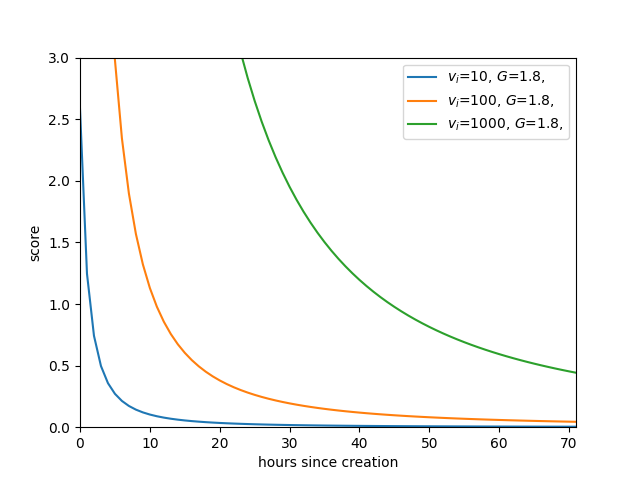
\includegraphics[width=\textwidth]{images/time_ranking_1.png}
    \caption{different views number}
  \end{subfigure}
  \hfill
  \begin{subfigure}[b]{0.5\textwidth}
    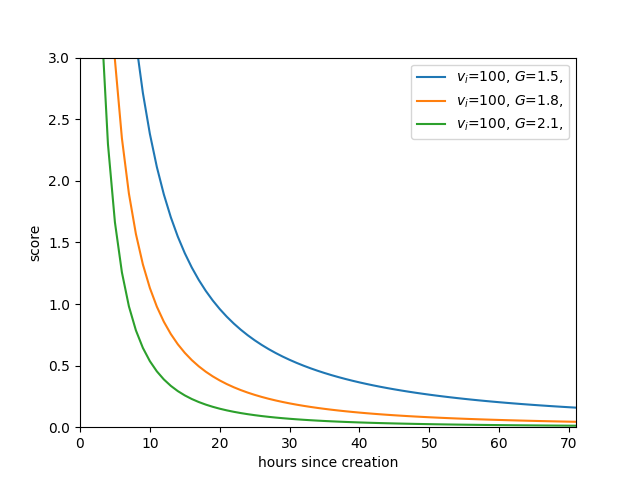
\includegraphics[width=\textwidth]{images/time_ranking_2.png}
    \caption{different gravity factor}
  \end{subfigure}
\caption{time-based ranking scoring}
    \label{fig:samples}
\end{figure}


At the end scores are normalized by \texttt{min-max} normalization.


\subsubsection{Content-based filtering (categories)}
\label{content}

We are representing each news item as a vector of confidence values (how strong each item belongs to category).

\begin{table}[h]
    \centering
    \begin{tabular}{cccccc}
        \toprule
        item\_id & \textit{politics} & \textit{IT} & \textit{social\_media} & $\cdots$ & \textit{confilcts} \\
        \midrule
        1 & 0.55 & 0 & 0 & $\cdots$ & 0.3 \\
        2 & 0    & 0.81  & 0.62 & $\cdots$ & 0 \\
        \vdots & \vdots & \vdots & \vdots & \vdots & \vdots\\

        \bottomrule
    \end{tabular}%
    \caption{text vectors}
    \label{tab:text_vectors}
\end{table}

Tagging is made in the following way: we have a dictionary of words that belongs to categories:

\begin{table}[h]
    \centering
    \begin{tabular}{cc}
        \toprule
        \textit{word} & \textit{category} \\
        \midrule
        trump & politics \\
        crash & accident \\
        telegeram & IT \\
        \vdots & \vdots \\
        \bottomrule
    \end{tabular}%
    \caption{words' categories}
    \label{tab:words_categories}
\end{table}

Confidence is taken from word's tf-idf metric alongside all corpus.

There is limited number of words, but during the day new words are being added and every night item vectors are being recalculated.

As user interacts with the system, we are forming his preferences vector in the following way:

\begin{equation}
    \texttt{user\_vector} \mathrel{+}= \texttt{action\_score} * \texttt{item\_vector}
\end{equation}

User vector has same dimension as item vector.

Where action score is taken from table:

\begin{table}[h]
    \centering
    \begin{tabular}{cc}
        \toprule
        \textit{action} & \textit{score} \\
        \midrule
        shown but now viewed & -1 \\
        viewed & 0.5 \\
        emoji or comment & 0.5 \\
        read till the end & 1 \\
        \bottomrule
    \end{tabular}%
    \caption{actions' scores}
    \label{tab:action_score}
\end{table}

As we now have both user's and items' vectors, we are able to find similarities between them:

\begin{equation}
    r_i = 1 - \cos{(\texttt{user\_vector}, \texttt{item\_vector})}
\end{equation}


As was told before, content-based filtering have its own impact weight, which is small at start (we don't want to restrict user from content just because he made some random clicks), but it inscreases as user interacts with the system and we may make predictions about his categorial preferences.

\subsection{Ranking components overview}



\subsubsection{Collaborative filtering}

We are using SVD++ algorithm.

For collaborative filtering recommendation we should have something known as user-item matrix which may be formed from user activity from tables (cite tables).

We use the modification of Funk MF, which factorized the user-item rating matrix as the product of two lower dimensional matrices, the first one has a row for each user, while the second has a column for each item. The row or column associated to a specific user or item is referred to as latent factors.

$r_{u i}=\sum_{f=0}^{n } H_{u, f} W_{f, i}$

While Funk MF is able to provide very good recommendation quality, its ability to use only explicit numerical ratings as user-items interactions constitutes a limitation. Modern day recommender systems should exploit all available interactions both explicit (e.g. numerical ratings) and implicit (e.g. likes, purchases, skipped, bookmarked). To this end SVD++ was designed to take into account implicit interactions as well.  Compared to Funk MF, SVD++ takes also into account user and item bias.
The predicted rating user $u$ will give to item $i$ is computed as:

$r_{u i}=\mu+b_{i}+b_{u}+\sum_{f=0}^{n} H_{u, f} W_{f, i}$

\subsubsection{Popularity filtering}

For measuring news item popularity following data can be aggregated: \hyperref[tab:show]{shows}, \hyperref[tab:view]{views}, \hyperref[tab:emotion]{emotions}, \hyperref[tab:comment]{comments}.

\begin{table}[h]
    \centering
    % \resizebox{\textwidth}{!}{
    \begin{tabular}{ccccc}
        \toprule

        \emph{item\_id} & \emph{shows\_num} & \emph{views\_num} & \emph{emotions\_num} & \emph{comments\_num} \\\midrule

        1 & 1043 & 231 & 52 & 7  \\
        2 & 828  & 478 & 78 & 11 \\
        3 & 163  & 25  & 5  & 0  \\
        \vdots & \vdots & \vdots & \vdots & \vdots \\\bottomrule


     \hline
    \end{tabular}
    % }

    \caption{aggregated popularity data}
    \label{tab:popularity}
\end{table}

So when we apply information about news item popularity, we are able to give them scores via following algorithm:

\texttt{min-max} normalizing each of \emph{shows\_num}, \emph{views\_num}, \emph{emotions\_num}, \emph{comments\_num}, then dividing by 4 (to have 1 as max after sum), and sum all of these values.


\subsubsection{Content-based filtering (LDA)}

For Content-based filtering we should somehow vectorize news items and represent user preferences via these vectorized news. We will use Latent Dirichlet Allocation (LDA), which is a generative statistical model that allows sets of observations to be explained by unobserved groups that explain why some parts of the data are similar. For example, if observations are words collected into documents, it posits that each document is a mixture of a small number of topics and that each word's presence is attributable to one of the document's topics.

So we are able vectorize text by the measure of how each text belongs to each category, from 0 to 1.
For example, suppose we have 3 topic, that were extracted by LDA model:

\begin{itemize}
    \item \textbf{Topic 1:} ruble, bank, money, dollar
    \item \textbf{Topic 2:} cooking, sugar, gordon\_ramsay
    \item \textbf{Topic 3:} IT, smartphone, technology, hacker
\end{itemize}

And we have following text: ``Hackers use mobile emulators to steal millions of dollars''. Its vectorized form is going to be $[0.7, 0, 0.8]$.

All calculations are done as was told in \ref{content}.


\subsubsection{Session filtering}

We want to instantly react on user's actions, so we applying session filtering in the following way:
trying to find similar item to those, user have just watched. So 

$$r_{i}=\sum_{k=0}^{n} \textit{similarity}\{\textit{current\_item\_vector}, \textit{last\_viewed\_vector}_{k}\} \times \textit{weight}_k$$

where $\textit{weight}_k$ is the weight of last viewed vector. Weight is bigger if item was seen more recently.



% \section{Implementation}
% \label{sec:implementation}

\section{Evaluation}
\label{sec:evaluation}

    For evaluation we have information about what recommendation list was given to each user, and what is the source of the recommendation:

    \begin{table}[h]
        \centering
        \begin{tabular}{cccc}
            \toprule
            \textit{user\_id} & \textit{recommendation\_list}       & \textit{content\_based\_filtering}  & \textit{collaborative\_filtering} \\
            \midrule
            2 & \{(2, 0.91), (1, 0.74), (3, 0.23)\} & \{(2, 0.45), (1, 0.54), (3, 0.08)\} & \{(2, 0.92), (1, 0.4), (3, 0.3)\}\\

            1 & \{(3, 0.73), (1, 0.69), (2, 0.15)\} & \{(2, 0.6), (1, 0.44), (3, 0.04)\} & \{(2, 0.58), (1, 0.58), (3, 0.14)\}\\
            \vdots & \vdots & \vdots & \vdots \\
            \bottomrule
        \end{tabular}%
        
        \caption{recommendations' logs}
        \label{tab:recommendation_logs}
    \end{table}

    \begin{itemize}
        \item \textit{recommendation\_list}: list of recommendations that consists of pairs (\textit{item\_id}, \textit{score})
        \item \textit{content\_based\_filtering \& collaborative\_filtering}: sources of recommendation
    \end{itemize}

    As we use weighted sum of our recommmenders, we have unique boost values for every user:

    \begin{table}[h]
        \centering
        \begin{tabular}{ccc}
            \toprule
            \textit{user\_id} & \textit{content\_based\_filtering} & \textit{collaborative\_filtering} \\
            \midrule
            1                 & 0.25                                  & 1                               \\
            2                 & 1                               & 0.5                                \\
            \vdots & \vdots & \vdots \\
            \bottomrule
            \end{tabular}%
        \caption{boost values}
        \label{tab:boost_values}
    \end{table}

    To illustrate score calculation of recommendations, take a look at 1st row of table \hyperref[tab:recommendation_logs]{recommendations' logs}. We see recommendation $r = \{(2, 0.91), (1, 0.74), (3, 0.23)\}$ for user $u = 2$, so we should find boost values for this particular user in table \hyperref[tab:boost_values]{boost values}: content-based filtering boost $b_{cbf}$ for $u$ is $1$, collaborative filtering boost $b_{cf}$ is $0.5$. So final score is calculated in the following way: $0.91 = 0.45 * b_{cbf} + 0.92 * b_{cf} = 0.45 * 1 + 0.92 * 0.5 = 0.45 + 0.46$.

    Also we have information about \hyperref[tab:show]{shows} and \hyperref[tab:view]{views}, so we are able to track what item in recommendation list was clicked and what item was skipped, so depending on this information we can track if user liked item or not.

    So having all of this information allows us to tune the impact weight of each recommender using grid search.



% \subsection{Online}

% \subsection{Offline}

% \section{Further research}
% \label{sec:further}

\section{Summary}
\label{sec:summary}


Recommendation system has been widely used in different areas. Collaborative filtering focuses on rating, ignoring the features of items itself. In order to better evaluate customer preference on news, we use LDA model to
calculate customer preference on news topics.

In order to forecast rating on news, we take similarity of customers and correlation between customers and news into consideration. Experiment shows that our hybrid recommendation method based on features performances better in our social media app.

What we contribute is we proposed a new hybrid recommendation method based on features to improve the performance.

Results show that combining different approaches leads to rise of users' involvement.

We use the average method to set the weight to adjust the predicted rating in this article, whose rationality needs to be further improved. Moreover, our method has yet to be tested on other data sets for its performance.  

\bibliographystyle{unsrtnat}
\bibliography{references}  

\end{document}
